\documentclass[uplatex,10pt,a4j]{jsarticle}
%\documentclass[10pt]{ujarticle}
\usepackage[top=30truemm, bottom=30truemm, left=25truemm, right=25truemm]{geometry}
\usepackage{listings}
\usepackage{ascmac}
\usepackage{amssymb}
\usepackage{amsmath}
\usepackage{bm}
\usepackage{url}
\usepackage[dvipdfmx]{hyperref}
\usepackage[dvipdfmx]{graphicx,color}
%ktaniguc insert
\usepackage[cc]{titlepic}
\usepackage{wallpaper}
%ktaniguc end
%\usepackage[dviout]{graphicx}
\lstset{
language=c,
basicstyle=\ttfamily\footnotesize,
commentstyle=\textit,
classoffset=1,
keywordstyle=\bfseries,
frame=tb,
framesep=5pt,
showstringspaces=false,
numbers=left,
stepnumber=1,
numberstyle=\tiny,
tabsize=2,
breaklines = true,
lineskip=-0.5ex
}


\begin{document}
\begin{titlepage}
  %\ThisCenterWallPaper{1}{TenkiNoKo_Titlepage.png}
  %\oddsidemargin=-50mm
  \title{SummerChallenge2021 \\ \Huge 量子の波動性と粒子性}

  %\topmargin=170mm
  \author{教員 : 山崎祐司, 河野能知, 宮林謙吉 \\TA : 楠戸愛美, 濱田悠斗, 山下智愛}
  %\titlepic{\includegraphics[width=12cm]{TenkiNoKo_Hyoushi.png}}
  \date{2022年3月5日〜9日}
  \maketitle
\end{titlepage}

\tableofcontents
\clearpage

\section{目的}
光には、波動性と粒子性の2重性がある。今回の実験では、光の粒子性または波動性のどちらか一方が顕著に現れる現象ではなく、光が両方の性質を同時にもっていると考えざるを得ないということを検証する。

\section{演習内容}

\subsection{演習1 光子を見る}
まずは干渉縞を観測する前に、そのために用いる実験装置の使い方や仕組みを学ぶために簡単に光子の測定を行う。今回の実験では光源としてLED,検出器としてMPPC,EASIROCを用いる。それぞれの詳しい説明は後で述べるためここでは省略するが、演習1でそれぞれの使い方を理解することを目的とする。
\begin{itemize}
  \item LEDをパルスジェネレータを用いて光らせ、それがきちんと光っていることを目視で確認する。
  \item MPPCで光子を観測する。そのためにはEASIROC,DELAY,DISCRIMINATORといったモジュールの使い方を理解して、さらにEASIROCの操作方法を理解する。
  \item データを解析する。ここで簡単なROOTの使い方を理解する。
\end{itemize}

\subsection{演習2 干渉縞を観測する}
今回の実験のメインテーマとなるスリットを用いた干渉縞の観測を行う。この演習では、干渉縞を観測できるセットアップとその結果の解析がメインになると思う。
\begin{itemize}
  \item レーザーポインタを用いてスリットの干渉縞を目視で確認する。実際の測定は暗箱内で行うため、常にこの干渉縞を観測しているとイメージしながら以降の測定を行ってほしい。
  \item 2重スリットを用いた干渉実験。まずは干渉縞がMPPCで観測できるようなセットアップにし、稼働ステージでMPPCを移動させながら測定を行う。1回の移動で動かす距離は、理論式から明線と暗線の間隔を計算し、そこから決めるとよい。
  \item ROOTを用いて測定データを解析して、干渉縞のグラフを描く。具体的な流れについては後で説明するためここでは省略する。
\end{itemize}

\subsection{演習3 1光子の干渉縞を測定する}
演習2からの変化として光子数を減らして、1光子数での干渉縞の観測を目指す。解析手法はほとんど変わらず、光量を抑える工夫をすればよい。基本的にはLEDへの印加電圧を下げれば光量は減少するが、それでも足りなければ各自で工夫してみてください。

\clearpage
\section{原理}

\subsection{光とは}
電子のエネルギー状態が、高エネルギー状態から低エネルギー状態へ変化した時、このエネルギーの差分を原子の外に波動エネルギーとして放出する。この波動エネルギーを電磁波・光と呼ぶ。
位置$\bm{r}$、時間tにおける電磁波は以下の式で表される。
\begin{itemize}
  \item 電場:$\bm{E} (\bm{r}, t) = \bm{E_0} \sin (\omega t - \bm{k} \cdot \bm{r} ) $
  \item 磁場:$\bm{B} (\bm{r}, t) = \bm{B_0} \sin (\omega t - \bm{k} \cdot \bm{r} ) $
\end{itemize}
$\bm{E_0}, \bm{B_0}$:定数、 $\bm{k}$:波数ベクトル、 $\omega$:角振動数とする。

\subsection{光の干渉}
光の波動性を見る1つの実験として、干渉実験がある。以下、光の干渉の原理について述べる。
\subsubsection{線状光源}
直線に並んだ振幅、周波数が互いに等しいN個の光源を考える。各光源は等しい初期位相角をもっていると仮定する。ここで、j番目の光源が$r_j$離れた点で作る電場$E_j$は
\[
  E_j = E_0 \sin(\omega t - k r_j)
\]
と書ける。今、$E_0 \varpropto 1/{r_j}$なので、定数$C_0$を用いて
\[
  E_j = \frac{C_0}{r_j} \sin(\omega t - k r_j)
\]



さらに、この光源を無限に並べた線状光源を考える。ここで、考えている状況は、各光源は非常に弱く、光源の数Nは極めて多く、光源間の間隔が無視できるほど小さい状況である。ここで、Dを線状光源全体の長さとすると、線状光源の微小部分$\delta y_i$個の光源を含んでいる。(ここで、光源はM個の微小部分に分けられているとする。$1 \leq i \leq M$)
\\
\begin{figure}[b]
  \begin{center}
    \includegraphics[width=6cm, bb = 0 0 600 200]{SummerChallenge_lineray.png}
    \caption{線状光源}
  \end{center}
\end{figure}

\clearpage
このとき$\delta y_i$がPに作る電場は、
\[
  E_i = \frac{C_0}{r_i} \sin(\omega t- k r_i ) \frac{\delta y_i N}{D}
\]
となる。ただし、$\delta y_i$は微小であり、この微小範囲内の各光源からPまで距離は一定であるとする。さらに一定値の$C_L$を
\[
  C_L = \frac{1}{D}  \lim_{N \to \infty} (C_0 N)
\]
と定義できる。M個の全部分によるPでの電場は、
\[
  E = \sum_{i=1}^M \frac{C_L}{r_i} \sin(\omega t - k r_i) \delta y_i
\]
最後に、$\delta y_i$は無限小になるはずで、
\[
  E = C_L \int_{-D/2}^{D/2} \frac{\sin(\omega t - k r)}{r} dy
\]
となる。ここで、$r = r(y)=\sqrt{R^2 \cos^2 \theta + (R\sin \theta - y )^2}$である。


\subsubsection{単スリット}
まず、単スリットの場合どのように干渉が起こるかを確かめる。振幅、周波数が互いに等しい長さDの線状光源を考える。線状光源の中心からyだけ離れた光源の微小部分dyが、中心からxy平面上の角$\theta$の方向にRだけ離れた点Pに作る電場は、
\[
  dE = \epsilon \frac{\sin(\omega t - kr)}{r} dy
\]
$r(y)$を$y$でテイラー展開すると、
\begin{eqnarray*}
  r &=&r(0) + \frac{\partial r(0)}{\partial y} y + \frac{1}{2!} \frac{\partial^2 r(0)}{\partial y^2} y^2 + \cdots \\
  &=&R - y\sin\theta + \frac{y^2}{2R} \cos^2 \theta
\end{eqnarray*}
となる。いま、$R \gg y$なので、第3項以降は無視できる。
\[
  dE = C_0 \frac{\sin(\omega t -k(R- y\sin \theta ))}{R- y \sin\theta} dy
\]
これの分母は$R \gg y$より$R$としてよいので、
\[
  dE = C_0 \frac{\sin(\omega t -k(R- y\sin \theta ))}{R} dy
\]
これは、Rが十分大きいとき、$\theta$の全ての値に対して正しい。
\begin{eqnarray*}
  E &=& C_L \int_{-D/2}^{D/2} \frac{\sin(\omega t - k( R - y\sin\theta ))}{R} dy \\
  %&=& \frac{C_L}{R} \int_{-D/2}^{D/2} sin(\omega t - k( R - ysin\theta )) \\
  &=& \frac{C_L}{R(kD/2)\sin\theta} \sin\left(\frac{kD}{2} \sin \theta \right) \sin(\omega t -kR) \\
  &=& \frac{C_L D}{R\beta} \sin \beta \sin(\omega t - kR)
\end{eqnarray*}
$\beta = \frac{kD}{2} \sin\theta$とすると、以上のようになり、線状光源が作る電場が導かれた。このとき、強度は$I(\theta) = \langle E^2\rangle_T$で求められるので、
\begin{eqnarray*}
  I(\theta) &=& \langle E^2 \rangle_T\\
  &=& \langle \sin^2(\omega t - kR)\rangle_T \left(\frac{C_L D}{E}\right)^2 \left(\frac{\sin\beta}{\beta}\right)^2
\end{eqnarray*}
$\langle E^2\rangle_T$は$E^2$の十分に長い時間発展で、周期 $2\pi / \omega$とすると、
\begin{eqnarray*}
  \langle \sin^2(\omega t - kR)\rangle_T  &=& \frac{\omega}{2\pi} \int_{0}^{2\pi / \omega} \sin^2(\omega t - kR) dt \\
  %&=& \frac{\omega}{2\pi} \int_{0}^{2\pi / \omega} \frac{1}{2} (1-cos(2(\omega t -kR))) dt \\
  &=& \frac{1}{2}
\end{eqnarray*}
より、
\[
  I(\theta) = \frac{1}{2} \left(\frac{C_L D}{R}\right)^2 \left(\frac{sin \beta}{\beta}\right)^2
\]
$I(0)$を求めると
\[
  I(0) = \frac{1}{2} \left(\frac{C_L D}{R}\right)^2
\]
なので、
\[
  I(\theta) = I(\theta) \left(\frac{\sin \beta}{\beta}\right)^2
\]
と求まる。光の強度の変化と観測位置の関係は以下のように表される。\\

\begin{figure}[h]
  \begin{center}
    \includegraphics[width=10cm, bb = 0 0 1000 800]{SummerChallenge_slit.png}
    \caption{単スリットでの光の強度と角度の関係}
  \end{center}
\end{figure}

\clearpage

\subsubsection{2重スリット}
図のような、幅$b$、中心間隔$a$の2本の長いスリットがあるとする。スクリーン上のある点の光波に対する式を得るには、2つの電場の和になるので、
\begin{eqnarray*}
  E &=& \frac{C_L}{R} \int_{-b/2}^{b/2} F(z) dz + \frac{C_L}{R'} \int_{a-b/2}^{a+b/2} F(z) dz \\
  &\simeq& \frac{C_L}{R} \int_{-b/2}^{b/2} F(z) dz + \frac{C_L}{R} \int_{a-b/2}^{a+b/2} F(z) dz \\
\end{eqnarray*}
ここで、
\begin{eqnarray*}
  F(z) &=& \sin(\omega t - k(R-z\sin\theta)) \\
  \alpha &=& \frac{ka}{2} \sin\theta \\
  \beta &=& \frac{kb}{2} \sin\theta
\end{eqnarray*}
これより、この式を簡単にすると、
\[
  E = 2 \frac{C_L b}{R} \frac{\sin\beta}{\beta} \cos\alpha \sin(\omega t -kR + \alpha)
\]
であり、単スリットの時と同様に強度$I(\theta) = \langle E^2\rangle_T$を求めると、$I(\theta) = \frac{1}{2} (\frac{C_L b}{R})^2$より
\[
  I(\theta) = 4I_0 \left(\frac{\sin \beta}{\beta}\right)^2 \cos^2 \alpha
\]
となる。\\
\\
\\
\\
\begin{figure}[h]
  \begin{center}
    \includegraphics[width=8cm, bb = 0 0 400 300]{SummerChallenge_2slits.png}
    \caption{2重スリットでの光の強度と角度の関係}
  \end{center}
\end{figure}

\subsubsection{参考文献}
\begin{itemize}
  \item 「フーリエ光学(第3版)」森北博巳(森北出版株式会社)2012年初版
\end{itemize}
\clearpage


\subsection{光子を数える}
光量が極端に少なくなると、光は光子として離散的になり、その数を数えることができるようになる。「光子数を数える」ということで、光の粒子性を観測することができる。どのような機器で測定するかは、次章にて述べる。


\section{実験装置}
\begin{figure}[h]
  \begin{center}
    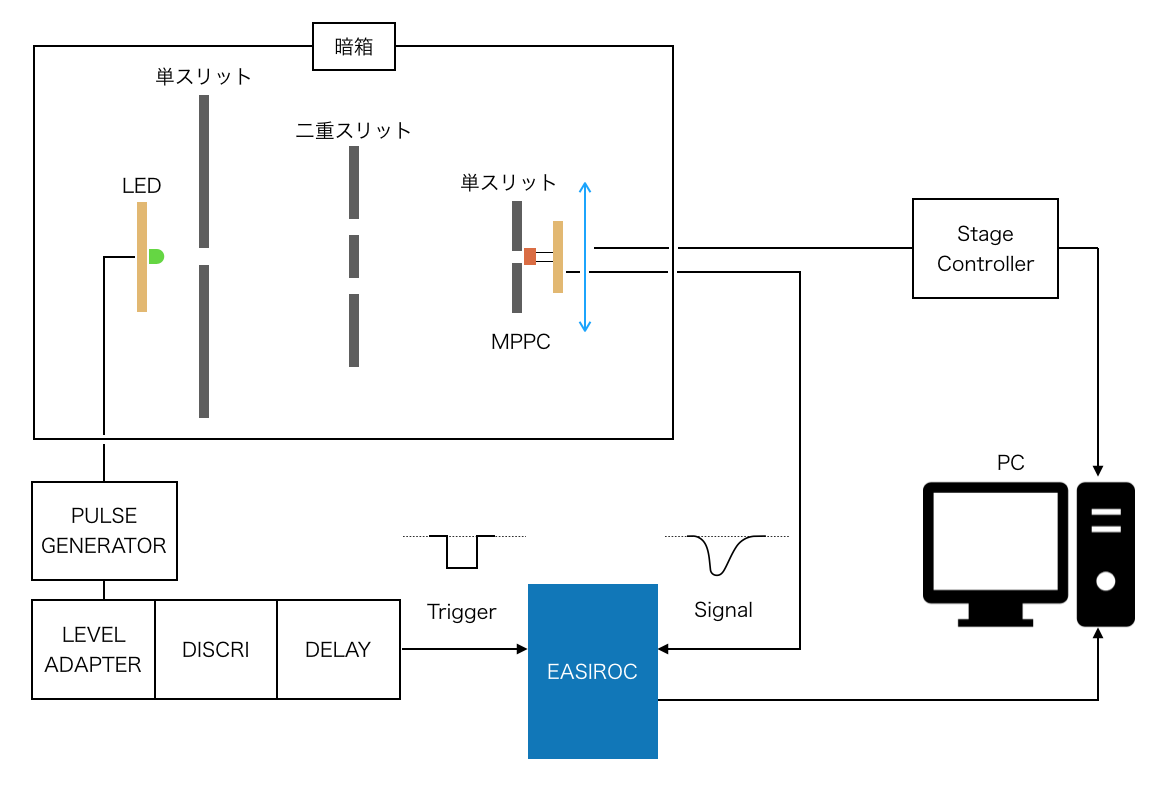
\includegraphics[width=12cm]{setup2019.png}
  \end{center}
  \caption{実験の模式図}
\end{figure}

本実験で用いる実験装置。
\begin{itemize}
  \item 光源(LED)
  \item 光検出器(MPPC)
  \item MPPC読み出しモジュール(EASIROC)
  \item スリット(単スリット・二重スリット)
  \item 可動式ステージ\par
        「Stage Controller」で制御。MPPCが設置されている基盤の位置を可動式ステージで細かく変更することが可能。
  \item 波高発生器(PULSE GENERATOR)\par
        非常に高い(1kHz)周期で矩形波を出力。出力と同期してトリガーを出力することも可能。
  \item レベルアダプター(LEVEL ADAOTER)\par
        TTL 入力信号をNIM 信号に変換し、出力。
  \item ディスクリミネータ(DISCRIMINATOR)\par
        アナログ入力信号の大きさがあるしきい値以上の場合に論理信号を出力。
  \item 遅延回路(DELAY)\par
        信号を遅らせるもの。要は長いケーブル。
  \item 測定用PC \par
        EASIROCの制御や、可動式ステージの制御を行う。データ取得まで行うことができる。
\end{itemize}
光学機器を図のように並べ、光の干渉を起こす。各デバイスの位置や距離によって干渉の見え方が変わるが、これは実際に物を置いていろいろ試してみるとよい。以下では、光検出器とその読み出しについて説明する。

\subsection{MPPC}
MPPC(Micro Pixel Photon Counter)はAvalamche Photo Diode(APD)が多数配列された光検出器である。APDは半導体でできている。P型とN型、異なるドープ型の半導体にある向きで電圧をかけると、キャリアの少ない空乏層ができる。ここに光子が入射すると、光電効果で電子をはじき出す。電子は印加電圧によってエネルギーを持ち、さらに周囲の原子殻内電子をはじき出し、雪崩(Avalanche)的に電子を倍増する。印加電圧によって様々な倍増モードがあるが、MPPC内のAPDでは、十分な印加電圧をかけることで入射光子数によらない出力電流を得る(ガイガーモード)。このガイガーモードAPDが多数配列することにより、我々は光子が入射したAPDのチャンネル数だけを数えることで、(pile upはあるものの)光子数をデジタルに数えることができる。
\begin{figure}[h]
  \begin{tabular}{ccc}
    \begin{minipage}[t]{0.33\hsize}
      \begin{center}
        \includegraphics[width=4cm]{mppc.jpg}
      \end{center}
      \caption{MPPC}
    \end{minipage}
    \begin{minipage}[t]{0.33\hsize}
      \begin{center}
        \includegraphics[width=4cm]{APDstructure.PNG}
      \end{center}
      \caption{APD}
    \end{minipage}
    \begin{minipage}[t]{0.33\hsize}
      \begin{center}
        \includegraphics[width=4cm]{QuenchingArray.PNG}
      \end{center}
      \caption{MPPCはAPDを並列に並べたもの}
    \end{minipage}
  \end{tabular}
\end{figure}
浜松ホトニクスのハンドブックに、詳細なMPPCの挙動が説明されている。\cite{hamamatsu}
\subsection{EASIROC}
EASIROCモジュールは、書き換え不可能な集積回路(ASIC)であるEASIROCチップと、EASIROCチップ制御用の書き換え可能な集積回路(FPGA)であるArtix7が搭載された、MPPCの(多チャンネネル)読み出しモジュールである。今回は1チャンネルしか使わないし、FPGAのfirmwareの書き換えも(おそらく)ないので、ここでは、EASIROCチップの回路の概要と、アナログな出力波形について見ることにする。\\
EASIROCチップは、Pre-Amp,Shaper,Discriminator,Capacitorからなる。Pre-Amp,Slow Shaperを通った信号電圧をCapacitorに保存し、Trigger信号が入力されたときに電圧をholdし、ADC(Analog Digital Converter)でデジタル情報に変換する。
\begin{figure}[h]
  \begin{center}
    \includegraphics[width=12cm]{EASIROCCircuitDiagram.PNG}
  \end{center}
  \caption{EASIROC回路概略}
\end{figure}

\begin{figure}[h]
  \begin{tabular}{cccc}
    \begin{minipage}[t]{0.25\hsize}
      \begin{center}
        \includegraphics[width=4cm]{preamp.BMP}
      \end{center}
      \caption{Pre-Amp}
    \end{minipage}
    \begin{minipage}[t]{0.25\hsize}
      \begin{center}
        \includegraphics[width=4cm]{fastshaper.BMP}
      \end{center}
      \caption{Fast Shaper}
    \end{minipage}
    \begin{minipage}[t]{0.25\hsize}
      \begin{center}
        \includegraphics[width=4cm]{slowshaper.BMP}
      \end{center}
      \caption{Slow Shaper}
    \end{minipage}
    \begin{minipage}[t]{0.25\hsize}
      \begin{center}
        \includegraphics[width=4cm]{slowshaperhold.BMP}
      \end{center}
      \caption{holdしたSlow Shaper}
    \end{minipage}
  \end{tabular}
\end{figure}


各デバイスを通った信号の出力波形は、EASIROCモジュールのProbe出力を観察するとわかる。Fast ShaperはSelf Trigger用なので、今回は(おそらく)使わない。Trigger信号に合わせてShaperの波高の一番高いところが読み出されているのがわかる。Trigger信号とShaperの立ち上がりがきちんと合うかどうかはケーブルの長さやDelayモジュールによって操作できる。

\section{測定方法}

\subsection{可動式ステージの使用方法}

可動式ステージは、stage.pyを用いて制御する。使用するためのコマンドは、以下の通りである。
\begin{lstlisting}[caption=stage.pyのコマンド]
\$ python stage.py [コマンド]  
\end{lstlisting}

\begin{table}[htbp]
  \begin{center}
    \caption{stage.py コマンド一覧}
    \begin{tabular}{|l|l|l|} \hline
      入力コマンド & 使い方       & 動作                                      \\ \hline \hline
      -o           & -o           & left or right 側の原点に戻る              \\ \hline
      -r           & -r           & データリセット、現在地を原点とする        \\ \hline
      -mr          & -mr [整数値] & 今いるところから[整数値]パルス分+側へ移動 \\ \hline
      -ml          & -ml [整数値] & 今いるところから[整数値]パルス分-側へ移動 \\ \hline
      -pr          & -pr [整数値] & 絶対的な座標位置+[整数値]パルスへ移動     \\ \hline
      -pl          & -pl [整数値] & 絶対的な座標位置-[整数値]パルスへ移動     \\ \hline
      -s           & -s           & 動作停止                                  \\ \hline
      -q           & -q           & ステージの情報を表示                      \\ \hline
      -h           & -h           & コマンドの使い方表示                      \\ \hline
    \end{tabular}
  \end{center}
\end{table}

\begin{itembox}[l]{注意事項}
  \begin{itemize}
    \item 動く距離とパルスの関係は2μm/パルス。
    \item 一度の操作で送ることのできるコマンドは1つ。
    \item 複数送った場合、コマンド一覧の上から順に優先順位がついており、優先順位が最も高いものの動作を行う。
  \end{itemize}
  例えば、{\tt \$ ./stage.py -ml 1000 -mr 20000 -s -o +} とコマンドを送っても, {\tt -o} のみが認識される。
\end{itembox}


\subsection{EASOROCの使用方法}

\subsubsection{EASIROCモジュールへのアクセス}

\begin{lstlisting}[caption=EASIROCモジュールへのアクセス]
  \$ EASIROC/easiroc/easiroc 192.168.10.102 3
\end{lstlisting}
でEASIROCモジュールへのアクセスが可能になる。数字の部分はEASIROCのIPアドレス。

\begin{lstlisting}
\$ cd EASIROC/easiroc
\$ ./easiroc 192.168.10.102 3

\ I'm : 192.168.10.102
\ Please select
\ 1. Transmit SC
\ 2. Tranmit Read SC
\ 3. ASIC Initialize
\ 4. Transmit Probe
\ 5. Connection Close
\ 6. Start DAQ
\ 7. Debug
\ input # === >
\end{lstlisting}
{\tt ”Please select''} 以降の文字が表示されていればOK。以降でこれら7つのコマンドを使い分け、EASIROCを操作する。主な各コマンドの操作内容は次のようになっている。

\begin{table}[htbp]
  \begin{center}
    \caption{easiroc コマンド一覧}
    \begin{tabular}{|l|l|} \hline
      入力コマンド & 動作                                                     \\ \hline \hline
      1            & EASIROC 測定後でもオシロスコープで波形を見ることができる \\ \hline
      2            & どのチャンネルを出力するかを決める                       \\ \hline
      5            & 接続を切る                                               \\ \hline
      6            & 測定開始                                                 \\ \hline
    \end{tabular}
  \end{center}
\end{table}

今回はch.12から出力される信号のみを見るため、コマンド"2"の出番はない。

\subsubsection{印加電圧の設定}

EASIROC起動後に
\begin{lstlisting}[caption=印加電圧の設定]
  \$ cd EASIROC/easiroc/easiroc_UDPcontrol
  \$ ./udp102
\end{lstlisting}
を実行することで、印加電圧を設定することができる。udp102を実行する。(102はIPアドレスの最後のところ)
\begin{table}[htbp]
  \begin{center}
    \caption{UDPcontrol コマンド一覧}
    \begin{tabular}{|l|l|} \hline
      入力コマンド & 動作                                                            \\ \hline \hline
      1            & HighVoltageの設定(この時打った電圧が全チャンネルに反映される) \\ \hline
      2            & HighVoltageのステータス                                         \\ \hline
      3            & 実際にかかっている電圧                                          \\ \hline
      5            & exit                                                            \\ \hline
    \end{tabular}
  \end{center}
\end{table}

\begin{itembox}[l]{注意事項}
  \begin{itemize}
    \item easirocで接続してからudp102を起動
    \item 電流は正常な値で数uA 程度である。10 倍以上の電流が流れるようであればすぐにHighVoltage を0 にすること
    \item udp102を終了してからeasirocの接続を切る\par
          (切るときはHighVolの設定を0にしてから何度か2でステータスを確認して、4V程度になったことを確認してから切る)
    \item 1で電圧をかける前に変な電圧がかかっていないか2でステータスを確認する
  \end{itemize}
\end{itembox}

\subsubsection{EASIROC測定手順}

2つの実行ファイルを並行して操作する必要があるため、2つのウィンドウを立ち上げる。これらを今後、ウィンドウ1,ウィンドウ2と区別する。また、測定結果も測定時に同時に確認したい場合は、ウィンドウを3つ用意する。

\begin{enumerate}
  \item EASIROCモジュールへアクセスする(ウィンドウ1)
  \item 印加電圧を設定する(ウィンドウ2)
  \item ウィンドウ2でコマンド''2''を打って印加電圧を設定する。印加電圧は53.5から54V程度が好ましく、それ以上に設定するとMPPCに負担がかかるため極力上げないこと。
  \item ウィンドウ1でコマンド''1''→''2''を入力し、オシロスコープにて波形を確認する。
  \item ウィンドウ1でコマンド''6''を入力し、測定を開始する\par
        \begin{lstlisting}[caption=測定手順]
\ input # ===>6
\ Input output data file name : ファイル名.dat
\ Input total # of events =====> 欲しいイベント数
\end{lstlisting}
  \item 測定結果の確認\par
        別ウィンドウ(ウィンドウ3)にて、
        \begin{lstlisting}[caption=測定結果の確認]
\$ root
\ root[0] .L fullcheck6.C
\ root[1] fullcheck6(''ファイル名.dat'')
\ root[2] TBrowser tb
\end{lstlisting}
        TBrowserが起動するので,その中から{\tt ファイル名.root}を探してその中のch.12に保存されているプロットが測定結果。
\end{enumerate}
rootの使い方に関しては、6.4節を参照。\par
データの収集方法についても、詳しくはマニュアル参照。EASROCボードのそれぞれのチャンネルが何をするものかは、User Guideの1章を参照すること。2章には、EASIROCボードの制御法が記されている。User Guideに簡単な操作法が記されているが、ボード仕様書にはさらに細かい情報が載っているので、困ったら参照すること。
\section{データ解析}
\subsection{MPPCで取得されるデータの解析}
MPPCで取得されるデータはEASIROCによってtree形式で保存される。今回はこのデータをROOTを用いて解析を行う。ここから解析に必要なROOTの知識を簡単に説明するが、すべてを説明することはできないためわからない部分は各自調べるかTAに質問したりするようにしてください。

\subsection{データ解析用PCにログインする}
ここでは、自分のPCからLinuxにリモートでログインする方法を説明します。

\subsubsection{Windows Subsystem for Linux (WSL) を用いてLinuxを使う}
Windows10 以降で使用可能になった Windows Subsystem for Linux(WSL) は、 Windows10 から Linux の実行環境を実現するサブシステムです。簡単にいうと、 Windows のアプリケーションとして Linux を実行できます。

\vspace{1cm}
{\large \bf WSL の有効化}
\vspace{0.5cm}

まず、Windows 側で Linux Subsystem を有効化します。
\begin{enumerate}
  \item スタートボタンを右クリックし、「アプリと機能」をクリックします。
  \item 右上の「プログラムと機能」をクリックします。
  \item 左サイドバーの「Windows の機能の有効化または無効化」をクリックします。
  \item 「Windows Subsystem for Linux」を探して、チェックを入れます。
  \item 「OK」を押すと、インストールが始まります。インストール後、再起動します。
\end{enumerate}

\vspace{1cm}
{\large \bf Ubuntu のインストール}
\vspace{0.5cm}

\begin{enumerate}
  \item Microsoft Store で「WSL」と検索します。もしくは「Ubuntu」。
  \item アプリの中から「Ubuntu」を探し、インストールします。
  \item インストール作業が終わったら、スタートに追加される「Ubuntu」をを起動します。
  \item ユーザー名とパスワード を要求されるため、プロンプトに従って入力していきます。
\end{enumerate}
\begin{lstlisting}[caption=表示されるスクリプト例]
Installing, this may take a few minutes...
Please create a default UNIX user account. The username does not need to match your Windows username.
For more information visit: https://aka.ms/wslusers
Enter new UNIX username: [user name]
Enter new UNIX password: [password]
Retype new UNIX password: [password]
passwd: password updated succsessfully
Installation successful!
To run a command as administrator (user ``root''), use ``sudo''.
See ``man sudo_root'' for details.
\end{lstlisting}

\begin{enumerate}
  \setcounter{enumi}{4}
  \item パッケージのアップデート\\
        パッケージのアップデートは日々行ったほうが良いです。
\end{enumerate}
\begin{lstlisting}
sudo apt update
sudo apt upgrade
\end{lstlisting}

\vspace{1cm}
{\large \bf X window のインストール}
\vspace{0.5cm}

\begin{figure}[h]
  \begin{center}
    \includegraphics[width=14cm]{VcXsrv.png}
    \caption{VcXsrvのHP。Downloadをクリックします。}
  \end{center}
\end{figure}

Windows OS で X window (画像表示用・root用) を使用するため、「VcXsrv」をインストールします。
\begin{enumerate}
  \item \url{https://sourceforge.net/projects/vcxsrv/} にアクセスし、「Download」をクリックします。
  \item インストーラを起動し、オプションやインストール先などを指定してインストールします。
        \begin{itemize}
          \item Installation Option : 全てにチェックする。 (Full)
          \item Installation Folder : C:¥Program File¥VcXsrv
        \end{itemize}
  \item インストール作業が終わったら、スタートに追加される「VcXsrv」をを起動します。
  \item 起動するとウィザード画面が表示される。それぞれ選択し、設定を完了させます。
        \begin{itemize}
          \item Display settings : 好きなもので
          \item Client startup : 次へ (start no client)
          \item Extra settings : 次へ (Clipboard - Primary Selection, Native opengl
          \item Save configuration : 「Save configuration」をクリック
        \end{itemize}
  \item システムトレイにVcXsrvのアイコンが表示されていれば OK です。
\end{enumerate}
\begin{figure}[h]
  \begin{center}
    \includegraphics[width=14cm]{XQuartz.png}
    \caption{XQuartzのHP。dmgファイルをクリックします。}
  \end{center}
\end{figure}
macOS の場合は、「XQuartz」をインストールします。
\begin{enumerate}
  \item \url{https://www.xquartz.org/} にアクセスし、 dmg ファイルをダウンロードします。
  \item dmg ファイルを展開し、XQuartz.pkg をクリックして、起動します。
  \item インストーラに従って、XQuartz をインストールします。
  \item インストールが完了すると、/アプリケーション/ユーティリティ/ に XQuartz.app が作成されていますので、正常に起動するか確認します。
\end{enumerate}

\subsubsection{SSH接続でリモートログインする}
\begin{lstlisting}
\$ ssh -Y [user name]@[host.IP.Address]
\end{lstlisting}
これで、Linux サーバーにログインできます。

\subsection{ROOTのインストール方法}

ROOTとはCERNが開発したデータ解析のためのフレームワークです。
特によく使われる目的としてはヒストグラム・グラフを描く、任意の関数でフィットする、大量のデータを処理するといったものがあります。
物理学実験では大量のデータを扱うため、例えばエクセルのようなものではそれらのデータをプロットしたり複雑な解析を行うことは難しくなります。
そのため、プログラミングによる解析を行えるようになる必要となります。
言語としては主にC++で動作し、pythonで書くこともできます。

\subsubsection{ROOTビルドの準備}

\vspace{1cm}
{\large \bf Windows版}
\vspace{0.5cm}

\vspace{0.5cm}
パッケージの準備
\vspace{0.3cm}

ROOTをUbuntu上で動かすにはあらかじめいくつかのパッケージをインストールしておく必要があります。次のURLにあるUbuntuのところのパッケージをインストールしてください。(すでにされているものもあると思います。)\\
\url{https://root.cern.ch/build-prerequisites}\\
最低限下記のものはインストールしてください。
\begin{lstlisting}
sudo apt-get install git dpkg-dev cmake g++ gcc binutils libx11-dev libxpm-dev libxft-dev libxext-dev
\end{lstlisting}

\vspace{0.3cm}
ROOTのソースファイルをダウンロード
\vspace{0.3cm}

Ubuntu用にコンパイルしたファイル をCERNが用意してくれています。\\
ROOTソースファイルのダウンロードは以下のページから。\\
\url{https://root.cern.ch/downloading-root}
\\
「Latest ROOT Releases Pro」をクリックすると、ダウンロード可能なファイルの一覧が表示されます。\\
ダウンロードするディレクトリを作成します。
\begin{lstlisting}
mkdir local
\end{lstlisting}
次のコマンドで最新のバージョンのrootがダウンロードされます。
\begin{lstlisting}
cd local
git clone http://github.com/root-project/root.git
ls
-root
\end{lstlisting}
ROOTをbuildするディレクトリを作成します。
\begin{lstlisting}
mkdir root_build
ls
-root  root_build
cd root_build
\end{lstlisting}
cmakeを行い、ROOTの構築に必要なファイルを生成する。
\begin{lstlisting}
cmake ../root
\end{lstlisting}
cmakeの実行が終了し、問題なければbuildを開始する。
\begin{lstlisting}
cmake --build . [-- <options to the native tool>]
cmake --build . -- -jN
\end{lstlisting}
オプションは下記のサイトで確認。2つ目のコマンドですると、buildをスピードアップできる。Nは利用可能なコア数により2や4などの数字を打つ。\\
参考URL(\url{https://root.cern.ch/building-root})\\
下記のコマンドを打ってROOTが起動すればbuildに成功しています。
\begin{lstlisting}
source bin/thisroot.sh
root
\end{lstlisting}
\vspace{0.3cm}
パスを通す
\vspace{0.3cm}

Ubuntuの起動時に毎回thisroot.shが実行されるようにします。
\begin{lstlisting}
vim ~/.bashrc
\end{lstlisting}
のコマンドでエディタを開いたあと以下を追記
\begin{lstlisting}
#ROOT
. ~/local/root_build/bin/thisroot.sh
\end{lstlisting}
Ubuntuの起動時に.bashrcが読み込まれるようにします。
\begin{lstlisting}
vim ~/.bash_profile
\end{lstlisting}
のコマンドでエディタを開いたあと以下を追記
\begin{lstlisting}
if [ -f ~/.bashrc ]; then
        . ~/bashrc
fi        
\end{lstlisting}
一度Ubuntuを閉じてもう一度起動し、下のコマンドを入力してROOTが起動すれば成功です。
\begin{lstlisting}
root
\end{lstlisting}

\vspace{0.5cm}

\vspace{1cm}
{\large \bf Mac版}
\normalsize{}

\vspace{0.5cm}
{\bf Homebrewのインストール}
\vspace{0.3cm}

Homebrew は macOS 用のパッケージマネージャーです。
Homebrew で ROOT ビルドに必要な CMake をインストールします。\par
Homebrew を使うには、Xcode の Command Line Tools が必要になります。
ターミナルで次のコマンドを実行し、Xcode をインストールします。
\begin{lstlisting}
\$ xcode-select --install
\end{lstlisting}
インストーラーの指示にしたがって、インストールを完了させます。
正常にインストールされていることを確認するため、
\begin{lstlisting}
\$ xcode-select -v
\end{lstlisting}
を実行します。バージョンが表示されていればインストール完了です。\par
次に、Homebrew をインストールします。
\url{https://brew.sh/index_ja.html}
上記のURLにあるコマンドをターミナルに入力します。
\begin{figure}[h]
  \begin{center}
    \includegraphics[width=14cm]{Homebrew.png}
    \caption{HomebrewのHP画面。画面下のコマンドをコピーしてターミナル上で実行する。}
  \end{center}
\end{figure}
\begin{lstlisting}[caption=Homebrewインストール時のスクリプト]
...
==> Installation successful!
==> Homebrew has enabled anonymous aggregate formulae and cask analytics.
Read the analytics documentation (and how to opt-out) here:
https://docs.brew.sh/Analytics
==> Homebrew is run entirely by unpaid volunteers. Please consider donating:
https://github.com/Homebrew/brew#donations
==> Next steps:
- Run `brew help` to get started
- Further documentation:
https://docs.brew.sh
\end{lstlisting}

が表示されれば、インストール完了です。\par

\vspace{0.5cm}
{\bf CMakeのインストール}
\vspace{0.3cm}

Homebrew を用いて、CMakeをインストールします。
\begin{lstlisting}
brew install cmake
\end{lstlisting}
を実行すると、CMakeがインストールできます。

\subsubsection{ROOTビルド方法}

\begin{lstlisting}
\$ cd ~
\$ curl -O https://root.cern.ch/download/root_v6.16.00.source.tar.gz
\$ cd /usr/local
\$ sudo tar zxvf ~/root_v6.16.00.source.tar.gz

\$ cd /usr/local/root-6.16.00
\$ sudo mkdir obj
\$ cd obj
\$ sudo cmake ..

...
-- Configuring done
-- Generating done
-- Build files have been written to: /usr/local/root-6.16.00/obj 
\end{lstlisting}

ここまで出ればCMake完了です。

\begin{lstlisting}[escapechar=!]
\$ sudo make -j 8

...
[100%] Generating tutorials/hsimple.root
Processing hsimple.C...
hsimple : Real Time = 0.06 seconds Cpu Time = 0.05 seconds
(TFile *) 0x7f9f7cda9760
[100%] Built target hsimple 
\end{lstlisting}

ここまで出ればビルド完了です\footnote{\url{https://root.cern.ch/building-root}を参考にしてください。}。

\subsubsection{ROOTの環境設定}

bash

\subsection{ROOTを用いたデータ解析}

\subsubsection{ROOTの起動方法}
ROOTの起動方法はコマンドラインに以下のコマンドを入力するだけです。
\begin{lstlisting}
root
\end{lstlisting}
\begin{figure}[ht]
  \begin{center}
    \includegraphics[width=8cm]{ROOT_logo.png}
    \caption{ROOTのロゴ}
    \label{fig:ROOT_logo}
  \end{center}
\end{figure}
起動の度に図\ref{fig:ROOT_logo}が表示されるため、オプションをつけます。
\begin{lstlisting}
root -l
\end{lstlisting}
\begin{table}[ht]
  \caption{ROOT起動時のオプションの例}
  \centering
  \begin{tabular}{lcr}
    \hline
    オプション & 意味                                           \\
    \hline \hline
    -l:        & 起動時にロゴを表示しない                       \\
    -b:        & ヒストグラムやグラフのグラフィックを描画しない \\
    -q:        & スクリプトファイルを実行後自動でROOTが終了する \\
    \hline
  \end{tabular}
\end{table}
ROOTを終了したいときには、.qと入力すればROOTを終了させることができる。

\subsubsection{ヒストグラムの描き方}
rootを起動する際に、引数にrootファイルを指定することでrootの起動と同時にROOTファイルを開くことができる。例えば、今回測定結果をexample.rootという名前で保存しているとした場合、root example.rootとコマンドラインから入力することで測定データに簡単にアクセスすることができる。\ref{fig:open_ROOT}
\begin{figure}[h]
  \begin{center}
    \includegraphics[width=8cm]{SummerChallenge_open_root.png}
    \caption{rootファイルを開く}
    \label{fig:open_ROOT}
  \end{center}
\end{figure}

example.root内にさらにtreeという名前でtreeを作っている場合、tree-$>$''コマンド''という書き方をすることができる。それにより、簡単に測定データを確認したりヒストグラムを描くことができる。コマンドとしては例えば、tree-$>$Print$\left(\right)$やtree-$>$Scan$\left(\right)$があり、Printはデータの数や種類、変数の方を確認でき、Scanは1つ1つのデータを実際に確認することができる。
\begin{figure}[htbp]
  \begin{center}
    \begin{tabular}{c}

      \begin{minipage}{0.5\hsize}
        \begin{center}
          \includegraphics[clip, width=60mm]{SummerChallenge_tree_print.png}
          \hspace{1.6cm} (a)tree-$>$Print$\left(\right)$の実行例
        \end{center}
      \end{minipage}

      \begin{minipage}{0.5\hsize}
        \begin{center}
          \includegraphics[clip, width=60mm]{SummerChallenge_tree_scan.png}
          \hspace{1.6cm} (b)tree-$>$Scan$\left(\right)$の実行例
        \end{center}
      \end{minipage}
    \end{tabular}
  \end{center}
\end{figure}

今回treeの中身をPrintやScanで確認すると、いくつかのBranchがあると思う。\footnote{Branchとは言葉通り枝のようなもので、1つのEntryに対して様々なデータを詰め込むことができる。}そのうち今回adcというBranchのヒストグラムを描きたい場合、tree-$>$Draw$\left(''adc''\right)$と打つだけでヒストグラムを描くことができる。\footnote{今回、EASIROCでは32chのデータが配列としてadcのBranchに入っており、そのうちMPPCがつながっているのは30chのみなので、adc[30]のみをDrawすることで測定データのヒストグラムを描ける}
\begin{figure}[htbp]
  \begin{center}
    \begin{tabular}{c}

      \begin{minipage}{0.5\hsize}
        \begin{center}
          \includegraphics[clip, width=60mm]{SummerChallenge_tree_draw_adc.png}
          \hspace{1.6cm} (a)tree-$>$Draw(''adc'')の実行例
        \end{center}
      \end{minipage}

      \begin{minipage}{0.5\hsize}
        \begin{center}
          \includegraphics[clip, width=60mm]{SummerChallenge_tree_draw_adc30.png}
          \hspace{1.6cm} (b)tree-$>$Draw(''adc[30]'')の実行例
        \end{center}
      \end{minipage}
    \end{tabular}
    \label{fig:tree_draw}
  \end{center}
\end{figure}

ヒストグラムを書くときに、ただそのまま書くだけでなく様々な条件をかけることもできる。例えば、tree-$>$Draw(''adc*2'')とすれば、adcの値を2倍したヒストグラムを描くことができ、tree-$>$Draw(''adc'',''adc>900'')とすればadcが900より大きいイベントのみ描くことができます。この条件には、ほかのBranchを用いることもできtree-$>$Draw(''adc'',''adc\_l $>$ 1000 \&adc\_l $<$ 3000'')とすれば1000$<$adc\_l$<$3000のみのヒストグラムを描くことができる。ただし、ある程度複雑な条件になってくるとこの書き方をするのは難しくなってくるので、後述するマクロを書いてヒストグラムを描くことをお勧めする。

最後にtreeをそのままdrawする以外のヒストグラムの描き方として、Fillという方法がある。簡単な例として、自分でガウス分布に従う乱数を発生させてそれをヒストグラムに詰めるやり方を紹介する。
\begin{lstlisting}
    TH1D *h1 = new TH1D(''h1'',''h1'',50,-5,5);
    for(Int_t i = 0;i < 10000;i++){
     Double_t x = gRandom->Gaus();
     h1->Fill(x);
    }  
    h1->Draw();
 \end{lstlisting}
3行目でgRandomというものを用いてGauss分布に従う乱数を発生させ、それを4行目でFillというコマンドでh1のヒストグラムに詰めている。それをfor文で回して10000回詰めている。このヒストグラムをDrawすることでGauss分布に従うヒストグラムを描くことができる。今回は例として乱数をFillしたが、乱数の代わりに詰めたい値を詰めることで好きなヒストグラムを描くことができる。

\subsubsection{マクロの書き方}
簡単なマクロはコマンドラインに書いてヒストグラムを描くときと同じものを描くだけでよい。ただし、rootファイルを読み込む際には必要な手順があるので例としてそれを示す。
\begin{lstlisting}[basicstyle=\ttfamily\footnotesize, frame=single]
void macro(){
	TFile *file = new TFile("example.root");
	TH1D *h1 = (TH1D*)file->Get("adc");
	h1->Draw();
}
 \end{lstlisting}
というファイルを作り、ターミナル上でroot macro.cxxやrootを起動した後、.x macro.cxxとコマンドすることでこのマクロを実行できる。
データの解析には基本的にはROOT固有の知識はそれほど必要ではなく、c++の知識があれば充分であるため深くは説明しない。

もう一つ必要な知識として、詳しい解析を行う際にはBranchのデータをヒストグラムとしてではなく値として取り出す必要がある。そのためこれも簡単にではあるが、値としての取り出し方を説明する。

\begin{lstlisting}
void macro(){
    TFile *file = new TFile(inputfilename, "read"); 
    TTree *tree = (TTree*)file->Get("tree");
 
    Double_t adc[32]
    tree->SetBranchAddress("adc", &adc);
 
    const Int_t N = tin->GetEntries();
    for (Int_t ientry = 0; ientry < N; ientry++) {
     tree->GetEntry(ientry);    
     cout<<ientry<<''   ''<<adc[30]<<endl;
   }
}
 \end{lstlisting}

tree-$>$GetEntry(ientry)とすることで、ientry番目のイベントのadcを読み込んでおり、それをfor文で全イベント回すことで全データを読み込んでいる。今回のマクロではcoutで出力しているだけだが、その値をvectorや配列に詰めることで解析に用いることができる。

コマンドラインによる解析の仕方も一応説明しているが、測定直後にデータを簡単に確認したいといった場合を除いてはマクロを用いればよい。また、データを確認する場合でもTBrowser\footnote{ROOTを起動した後、TBrowser tbと入力することでrootファイルの中身をヒストグラムとして簡単に見ることができる}が便利であるため、あまり使用頻度は高くないと思われる。

\subsubsection{ヒストグラムのフィット}
ROOTにはあらかじめガウス分布やポアソン分布などの様々な関数が用意されており、それらをヒストグラムのフィットを行う際に利用できる。例えばガウス分布でフィットする際には、htemp-$>$Fit(''gaus'')とすればよい。\footnote{htempの部分はその時のヒストグラムの名前に応じて適宜変える}コマンドラインで行った場合にはコマンドラインにfitの結果が出力される。
\begin{figure}[h]
  \begin{center}
    \includegraphics[width=8cm]{SummerChallenge_fit_gaus.png}
    \caption{フィットの結果}
    \label{fig:fit_gaus}
  \end{center}
\end{figure}

ガウス分布の場合は、$(gaus)=(Constant)\times$exp$(-\frac{(x-(Mean))^2}{2(Sigma)^2})$で定義されている。それぞれの出力されるパラメータは関数によって異なるため、ほかの関数を用いる際は一度確認しておくとよい。
また、htemp-$>$Fit(''gaus'','''','''',min,max)とすることでフィットする範囲を制限することができる。

あらかじめ定義されている関数以外の関数を用いたい場合は自分で定義することができる。例えば直線でフィットしたい場合には、
\begin{lstlisting}
TF1 *f1 = new TF1(''f1'',''[0] + [1] * x'',min,max);
 \end{lstlisting}
とすることでまず直線の関数を定義することができる。この関数の名前はf1になっているので、あとは先ほどガウス分布でフィットしたときと同様に、
\begin{lstlisting}
htemp->Fit(''f1'','''','''',min,max);
 \end{lstlisting}
とすればよい。

フィットする際にある程度のパラメータを指定したい場合がある。その際にはf1->SetParameter(0,5)とすれば0番目のパラメータの初期値を5に設定でき、f1->SetParameters(5,10)とすればまとめて複数のパラメータの初期値を設定できる。

マクロで行う場合には基本的には同じだが、フィットした結果をマクロ内で用いたい場合は値として取り出す必要がある。
\begin{lstlisting}
Double_t p0 = f1->GetParameter(0);
 \end{lstlisting}
とすると、p0にフィットした後の0番目のパラメータの値を代入することができる。

\subsubsection{グラフの描き方}
基本的な使い方として、テキストファイルからグラフを描くやり方と配列やvector\footnote{vectorが何かわからない場合はc++の勉強が先に必要なため、c++ vector等で検索して使い方を勉強したほうがよいでしょう}を用いる方法がある。まずはテキストファイルでのグラフの書き方から説明する。

例としてdata.datというファイルに
\begin{lstlisting}
1.00 3936
0.50 3007
0.10 2249
-0.10 1836
-0.50 1097
-1.00 146
 \end{lstlisting}
と書かれている場合、簡単にグラフを描くことができ
\begin{lstlisting}
TGraph *tg1 = new TGraph(''data.dat'');
tg1->Draw(''AP'');
 \end{lstlisting}
とするだけでグラフを描くことができる。ただし、この方法を用いるためには結果をまずdatファイルとして出力する必要があるため、あまり使うことはないだろう。

配列やvectorを用いる場合、まずは配列やvectorにデータを詰める必要があり、その部分は省略する。すでに値が詰まっていると仮定すると、配列の場合は
\begin{lstlisting}
TGraph *tg1 = new TGraph(6,x,y);
tg1->Draw(''AP'');
 \end{lstlisting}
とすると、6個のデータを含むグラフを描くことができる。しかし、測定データによってグラフが何点あるかは異なる場合もあり、vectorを用いたほうが様々な場合に柔軟に用いることができ便利である。

vectorを用いた場合は
\begin{lstlisting}
TGraph *tg1 = new TGraph(x.size(),&(x.at(0)),&(y.at(0)));
tg1->Draw(''AP'');
 \end{lstlisting}
c++の知識がある人は、これを見てやってることは同じだとわかると思う。

また、グラフにエラーバーをつけたい場合も多いと思う。その場合はTGraphではなくTGraphErrorsを用いればよい。使い方はほとんど同じで、
\begin{lstlisting}
TGraph *tg1 = new TGraph(6,x,x_error,y,y_error);
tg1->Draw(''AP'');
 \end{lstlisting}
の順番に引数がなっており、その通りにTGraphの時と同様に配列やvectorで与えればよい。

最後にグラフのフィットについてであるが、ヒストグラムの場合と全く同じであり例えば直線でフィットしたい場合には
\begin{lstlisting}
TF1 *f1 = new TF1(''f1'',''[0] + [1] * x'',min,max);
tg1->Fit(''f1'','''','''',min,max);
 \end{lstlisting}
とすればグラフを直線でフィットすることができる。

\subsubsection{結果の保存}
コマンドラインで結果のヒストグラムやグラフを保存する場合には、左上のFileからSave Asを選ぶと名前を付けて保存することができる。マクロで実行している場合には、ヒストグラムやグラフを描く前に
\begin{lstlisting}
TCanvas *c1 = new TCanvas(''c1'',''c1'',1600,900);
 \end{lstlisting}
としてキャンバスを作っておき、ヒストグラムやグラフをDrawした後に
\begin{lstlisting}
c1->SaveAs(''save name'');
 \end{lstlisting}
とすることで保存することができる。保存する際にきれいにヒストグラムやグラフを整えた後、保存したい人も多いと思う。rootはヒストグラムやグラフそれぞれに様々な修飾等が存在し、それをここで説明しているときりがないためまとめ\ref{sec:lastsection}にそれらが書かれているリンクを載せておく。

また、ヒストグラムを保存する際に画像としてでなくrootファイルにヒストグラムのまま保存することができる。実際に触ってみないとそのメリットは感じにくいかもしれないが、rootファイルの状態で保存することで、保存した後にタイトルをつけたりbin幅を変えるといった加工が簡単に行える。そのため、最終的にスライド等に用いる時以外はrootファイルで保存しておいたほうが便利かもしれない。具体的なやり方が書かれているサイトのリンクをここに載せておく。\footnote{\url{https://www-he.scphys.kyoto-u.ac.jp/member/n.kamo/wiki/doku.php?id=study:software:root:io}のWrite ・オブジェクトをファイルに書き込む、rootファイルを保存するを参考にしてもらえばよい。}なお、ヒストグラム等を保存する際は測定データのrootファイルとは別に保存用のrootファイルを作るようにしてください。測定データを上書きしてしまうリスクを避けるために、測定データは読み込み専用で開く習慣をつけるためである。

\subsection{Poisson統計}
Poisson分布とはめったに起こらない事象を大量に測定した場合にこの分布に従うことが多い。式で表すと、
\begin{equation}
  P\left(n\right)=\frac{\lambda^n e^{-\lambda}}{n!}
\end{equation}
で、これは平均$\lambda$起こる事象がn回起こるときの確率を表す。今回の実験の場合はそれぞれの測定での光子数の分布はPoisson分布に従うと思われる。
\begin{figure}[h]
  \begin{center}
    \includegraphics[width=8cm]{SummerChallenge_poisson.png}
    \caption{poisson分布の図}
    \label{fig:poisson}
  \end{center}
\end{figure}

$\lambda$が大きい場合はPoison分布はGauss分布(正規分布)に従う。今回の実験の場合では、それぞれの光子数に対応するピークはGauss分布に従うと思われる。
\begin{figure}[h]
  \begin{center}
    \includegraphics[width=8cm]{SummerChallenge_gauss.png}
    \caption{gauss分布の図}
    \label{fig:gauss}
  \end{center}
\end{figure}

\subsection{干渉縞の再現}
今回の測定データは最初adcの値として保存されており、この値自体に物理的な意味はない。そのため、まずはこの値から光子数に変換する必要がある。やり方としてはそれぞれのピークが光子数に対応しているため、それぞれをガウス分布でフィットして中心値を求める。そのadc値と光子数の関係を直線近似することで横軸をadcから光子数に変換することができる。

そのあと、変換した後のヒストグラムからMPPCの位置ごとの平均光子数を求めてプロットすることで干渉縞を再現することができる。平均光子数については様々な求め方があるが、簡単なものについては光子数で重みづけした平均、もう少しちゃんと求める場合には上で述べたように光子数の分布はPoisson分布に従うため、全体をPoisson分布でフィットすることで求めるほうがよい。

また、演習3で光子数を減らした場合はフィットで平均光子数を求めることは難しい。その場合は平均光子数ではなく1光子以上のイベント数で考えるとよい。平均光子数そのものではないが、光子数が少ない場合には平均光子数に比例して1光子以上のイベント数も増加するため、それでも干渉縞を観測することができる。\footnote{物理的な説明をすると、1光子の干渉と仮定すると明線の部分では光子の存在確率が大きいため、光子を観測するイベント数が増加する。光子数が増加すると光子数0となるイベントは暗線であっても減少するため、この考え方で解析することは難しくなる。}

\section{まとめ}
\label{sec:lastsection}
今回説明できたのはごく基本的な部分のみであり、今回の実験の解析についてもこれ以上の知識が必要になることがあると思う。c++の知識でわからないことがあれば

\url{http://www7b.biglobe.ne.jp/~robe/cpphtml/}
の第1部を見ればある程度の情報はのっていると思われる。もし、これにのっていない知識が必要になれば別途調べるか質問してください。

ROOTについての情報は基本的なものは

\url{http://www-ppl.s.chiba-u.jp/~hiroshi/ref/ROOT_text.pdf}

\url{https://www.quark.kj.yamagata-u.ac.jp/~miyachi/ROOT/root.pdf}

、途中で話した修飾については

\url{http://atlas.kek.jp/comp/ROOT-commands.html}

を見ればある程度一覧になっている。もし、そこにのっていない知識が必要になったときは別途調べるか、

\url{https://root.cern.ch/guides/users-guide}

のUser's Guideを見ればわかると思うが、User's Guideは英語の上膨大であるため、適宜調べるのがよいと思う。

また、あまり全てを書きすぎると参加している皆さんが考えることがなくなってしまうため、あえて説明をしていない部分もある。なので、この資料を読んでわからないことがあれば遠慮せずにどんどん聞いてください。

\begin{thebibliography}{9}
  \bibitem{hamamatsu}
  https://www.hamamatsu.com/resources/pdf/ssd/03\_handbook.pdf
\end{thebibliography}
\end{document}
